\documentclass[conference]{IEEEtran}
\IEEEoverridecommandlockouts
% The preceding line is only needed to identify funding in the first footnote. If that is unneeded, please comment it out.
\usepackage{cite}
\usepackage{amsmath,amssymb,amsfonts}
\usepackage{algorithmic}
\usepackage{graphicx}
\usepackage{textcomp}
\usepackage{xcolor}
\def\BibTeX{{\rm B\kern-.05em{\sc i\kern-.025em b}\kern-.08em
    T\kern-.1667em\lower.7ex\hbox{E}\kern-.125emX}}
\begin{document}

\title{Paper Title*\\
{\footnotesize \textsuperscript{*}Note: Sub-titles are not captured in Xplore and
should not be used}
\thanks{Identify applicable funding agency here. If none, delete this.}
}

\author{\IEEEauthorblockN{1\textsuperscript{st} Given Name Surname}
\IEEEauthorblockA{\textit{dept. name of organization (of Aff.)} \\
\textit{name of organization (of Aff.)}\\
City, Country \\
email address}
\and
\IEEEauthorblockN{2\textsuperscript{nd} Given Name Surname}
\IEEEauthorblockA{\textit{dept. name of organization (of Aff.)} \\
\textit{name of organization (of Aff.)}\\
City, Country \\
email address}
\and
\IEEEauthorblockN{3\textsuperscript{rd} Given Name Surname}
\IEEEauthorblockA{\textit{dept. name of organization (of Aff.)} \\
\textit{name of organization (of Aff.)}\\
City, Country \\
email address}
\and
\IEEEauthorblockN{4\textsuperscript{th} Given Name Surname}
\IEEEauthorblockA{\textit{dept. name of organization (of Aff.)} \\
\textit{name of organization (of Aff.)}\\
City, Country \\
email address}
\and
\IEEEauthorblockN{5\textsuperscript{th} Given Name Surname}
\IEEEauthorblockA{\textit{dept. name of organization (of Aff.)} \\
\textit{name of organization (of Aff.)}\\
City, Country \\
email address}
\and
\IEEEauthorblockN{6\textsuperscript{th} Given Name Surname}
\IEEEauthorblockA{\textit{dept. name of organization (of Aff.)} \\
\textit{name of organization (of Aff.)}\\
City, Country \\
email address}
}

\maketitle

\begin{abstract}
This document is a model and instructions for \LaTeX.
This and the IEEEtran.cls file define the components of your paper [title, text, heads, etc.]. *CRITICAL: Do Not Use Symbols, Special Characters, Footnotes,
or Math in Paper Title or Abstract.
\end{abstract}

\begin{IEEEkeywords}
component, formatting, style, styling, insert
\end{IEEEkeywords}

\section{Introduction}
An increasing number of convenience stores as well as medium-scale and small-scale supermarkets appears in our surroundings.
To make a long-term profit, retailers desire to keep their overall cost as low as possible in terms of management, labor, logistics and properties.
According to the latest news, The Home Depot yearly labor cost 90,444 million, Costco yearly logistics cost 10,444 million.
Labor costs account for a large part of the operating costs of shopping malls.
So in recent years, many shopping malls have sought to transform and reduce labor costs with the same profits.
In recent year, there are many stores that require little or no manual labor, many stores have changed their business model..
They all use computer identification technology to reduce labor costs, and it has more advantages than traditional shopping malls.
They have quick checkout and self checkout technology, make people's shopping faster, make the management of operators more convenient.

Meanwhile, a concept of "cashier-free supermarket" is proposed in nowadays, which draws much public attention.
This technology is undoubtedly the best way to solve the labor cost at present, and over time it will gradually replace the traditional business model.
The number of unmanned supermarkets is increasing, and it is becoming an emerging business model in the future, for an instance,  the novel idea of “Take it away”as announced by Amazon Go.
Amazon Go, Sam's Club Now and Taocafe are three pioneers that jump into the "cashier-free supermarket" technology and make it come true.
Amazon Go already started 5 unmanned stores in U.S. and they are planning to open up to 1000 stores till 2020.
Sensors and camera scan detect the categories and quantities of the products that a customer takes, it can make a preliminary settlement the self operation problems.
Moreover, with a proper camera layout, more integrated information can be gathered to strengthen our estimation of the quantitative variation of the products\cite{ERDEM2006156}.
Camera monitoring the purchasing behavior is an important part in a "cashier-free supermarket", and the change from a traditional supermarket to an advanced supermarket can be achieved by upgrading the capabilities and layouts of cameras, to provide an identification feature.
This paper will discuss the techniques of the modern cameras, mainly about device layouts, items category identification and quantity counting.
And achieve the establishment of Recognition System, the technology used and the problems solved.
%layout to cover all scene suitable

The rest of this paper is structured as follows:

Section \ref{sec:rw} xxxx

Section \ref{sec:rw} xxxx

 xxxx in Section \ref{sec:rw}.



\section{Related Works}
\label{sec:rw}

Compare Amazon Go and Sam's club Now, Amazon Go stores utilize a combination of sensors on the shelves, cameras and computer vision with machine learning.Different from Amazon Go, Sam's Club Now pay more attention on camera layout to plan shopping routes, and it use RFID\cite{1192765}.In our experiment, we get their merits, we set camera layout first, then use computer vision and sensors to identity items category and quantity.

\subsection{Camera layout}

\subsection{Computer vision}
Two of the most popular computer vision are YOLO and Faster-RCNN. The both have strong recognition ability. Faster-RCNN is a technology for using CNN to research feature map, and use RPN network to do full join operation for this, then send it to box regression layer and taxonomy\cite{NIPS2015_5638}. YOLO input S×S grid, and every gird is responsible for the objects falling into it, then it can choose the maximal IOU of bounding box\cite{yolov3}. We choose YOLOv3 for our experiment, because in processing medium-scale and small-scale da

\subsection{Weight sensor}


\section{ Technical comparison }

\subsection{official tones}

\subsection{end-user comments}
https://play.google.com/store/apps/details?id=com.amazon.ihm.richard&showAllReviews=true
https://play.google.com/store/apps/details?id=com.samsclub.sng
https://play.google.com/store/apps/details?id=com.samsclub.now

ESL: electronic shelf label
small fontsize for elderly people

60yrs age grandma.
samsclub , membership fee.  self check-out on smartphones.  reduce cost, incurring burden onto customers.

younger adults, students
no line, quick, smartphone 

proofread





\section{Method}

We did a series of experiments to achieve "cashier-free supermarket".
Include make scene to simulate a real supermarket and use multi cameras to cover whole scene to get  images which used to identity items types and number on shelves.

\subsection{Multi cameras and Build scene}
We build the Multi cameras scene is based on field of view(FOV), the horizontal field of view(H-FOV) and vertical field of view(V-FOV)\cite{Ball88} determined the sharpness and size of the pictures what we get.

\begin{figure}[htbp]
\centerline{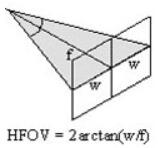
\includegraphics[width=2.5cm,scale=0.4]{HFOV.jpg} 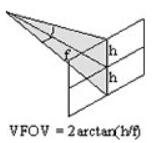
\includegraphics[width=2.5cm,scale=0.4]{VFOV.jpg}}
\caption{H-FOV and V-FOV .}
\label{fig}
\end{figure}

Fixed focal length lens, it can get the angel field of view(AFOV), and we can get different size of FOV through adjusting the focal length of the lens through different working distances.

\centerline{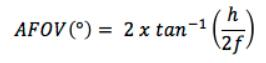
\includegraphics[width=5cm,scale=0.9]{AFOV-MA.jpg}}
\begin{figure}[htbp]
\centerline{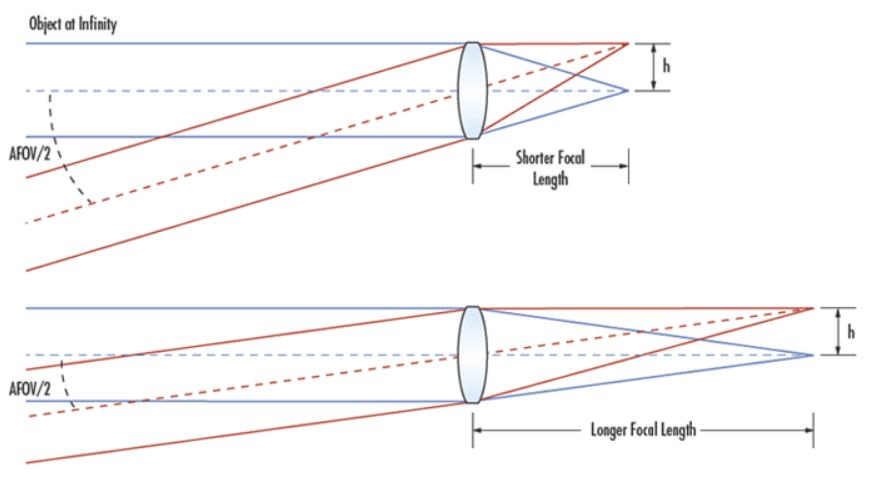
\includegraphics[width=9cm,scale=0.9]{AFOV.jpg}}
\caption{The field of view of lens is related to focal length, f is the focal length, h is the horizontal dimension of the sensor.}
\label{fig}
\end{figure}

We can follow the specifications of the scene (shelves size, the length and width of walking, and layout of the whole scene) to adjust FOV.

\subsection{Cameras selected}

The terms "dots per inch" (DPI) and "pixels per inch"(PPI) are used interchangeably by many. A 200 dpi print means that for each inch of that printed material, it takes about 200 dots to make the picture. A pixel is like a square dot without gaps. Both of them can describe the quality of a picture, and some cameras save digital images in arbitrary values as 72 dpi. We can calculate the DPI or PPI for what we need page size in Fig.3.
\begin{figure}[htbp]
\centerline{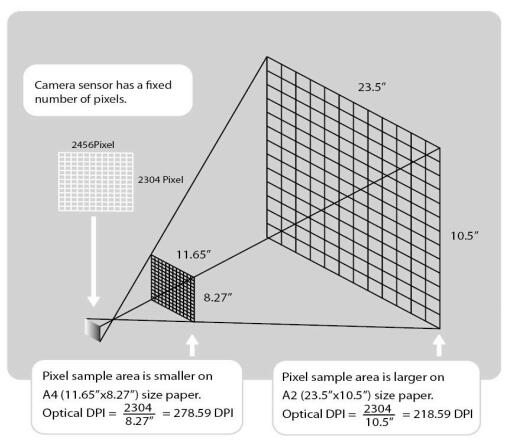
\includegraphics[width=8cm,scale=0.9]{DPIPPI.jpg}}
\caption{Page Size and Optical Resolution}
\label{fig}
\end{figure}

FLEXIDOME IP panoramic 7000 MP, which has 12MP / 30 fps sensor for fine details with smooth motion and Intelligent Video Analysis on full panoramic overview. Panoramic surveillance offers full 180° or 360° coverage of the designated area. The 360° version of the camera, when mounted
centrally on a ceiling, gives complete wall-to-wall coverage. The 180° version has a higher effective resolution and is ideal for wall mounting or for ceiling
mounting in corridors.

When mounted at a height of 3.5 m (11.48 ft) the 360° version of the camera has the following coverage radius for the four levels in Fig.4.
\begin{figure}[htbp]
\centerline{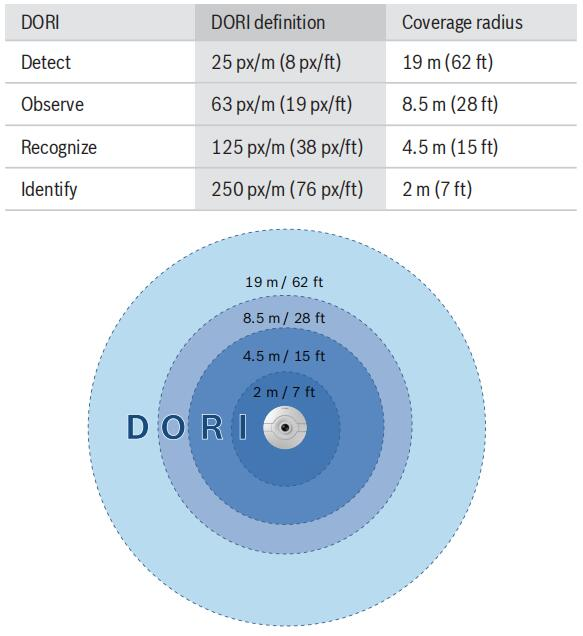
\includegraphics[width=7cm,scale=0.8]{camera360.jpg}}
\caption{Page Size and Optical Resolution}
\label{fig}
\end{figure}

When mounted at a height of 3.5 m (11.48 ft) the 180° version of the camera has the following coverage radius for the four levels in Fig.5.
\begin{figure}[htbp]
\centerline{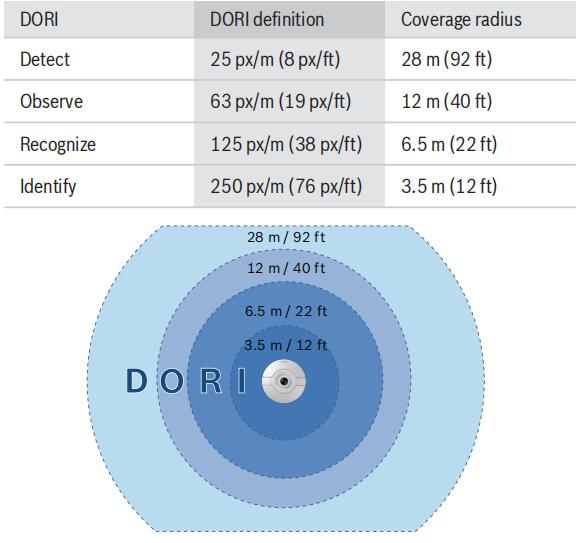
\includegraphics[width=7cm,scale=0.8]{camera180.jpg}}
\caption{Page Size and Optical Resolution}
\label{fig}
\end{figure}
The camera provides the full resolution circular image for recording even if we are viewing only a portion of the scene.

\subsection{Identity items}

A single GTX 1060 GPU has 6GB of memory, it is enough for us to train examples, therefore we spread the net across GPU. 
We can use the Python Reptile to get image from Internet, then use visual GUI-software for marking bounded boxes of objects and generating annotation files. 
It will create .txt-file for each .jpg-image-file in the same directory and with the same name, but with .txt-extension, and put to file: object number and object coordinates on this image, for each object in new line: object-class, x, y, width, height.

\subsection{Item Recognition}

\subsection{sensor fusion}


\section{Simulator}

In the previous section, we already introduce how to design scenarios and how to arrange them.
After we have explored and designed these necessary parameters.
Then in this section, we start with building up the scenarios described earlier.
It is included achieve the cashier-free supermarket in Unity3D, and the item recognition method what we use, then we combine them into a whole and application of simulation in real scene.

\subsection{Scene simulation}

Achieving our scene in Unity3D  which can simulate scene like a truth supermarket, the model is basic on the layout of Supermarket after our investigation.
It is length and width and height of the scene are 40m, 25m, 6m, and aisle width is 2.7m.
In the scene we set 5 bins, and each of bin width is 2.35m and height is 1.7m.
When have built the scene, we can design add the multi cameras to our scene, then put the cameras on the bins.
In the scene we put the each camera on the bins which height is 2.22m, it is through our calculation, the most conducive to obtaining the height of the image, and set cameras 6.8m apart from the previous calculations.
Then build four-direction cameras on the aisle, which is placed every 3 meters above the corridor, the cameras coverage needs to cover the entire scene.
A four-direction camera has 4 cameras for 4 directions, and we put them on the 3.5m. height of aisle.
In the scene we built, we totaly use 152 cameras in this scene.
The overall layout is shown in the Fig.8.

\begin{figure}[htbp]
\centerline{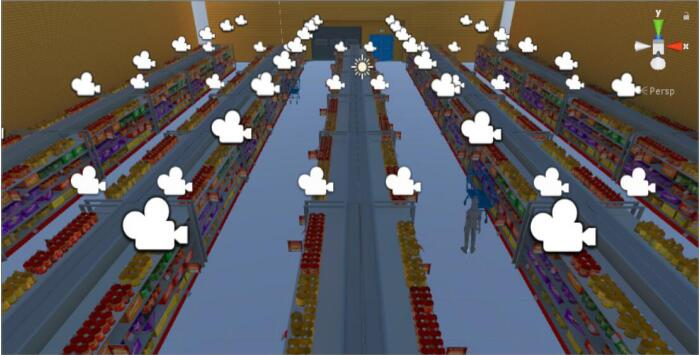
\includegraphics[width=7cm,scale=0.8]{supermarket.jpg}}
\caption{The whole simulated supermarket scene}
\label{fig}
\end{figure}

After setting up the scene, we also need to adjust the visual field and angle of each camera to get the best shooting pictures.
Through calculation and field investigation, we draw the h-fov is 1.2 bin is best for catching the maximum range and clearer picture, and the each camera can cover 2 bin.
In Fig.9, we can see the cameras which on shelves can clearly obtain the type and quantity of items, this provides a great help for our later identification.

\begin{figure}[htbp]
\centerline{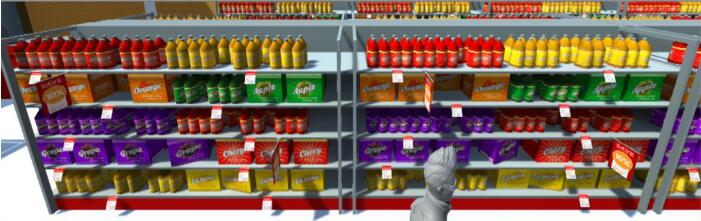
\includegraphics[width=7cm,scale=0.8]{shelves.jpg}}
\caption{Information on the shelf captured by camera shuttle}
\label{fig}
\end{figure}

The simulated scene is based on the real scene, it can serve as a reference.
In this scene, we can design the placement of cameras, and calculate the location of the camera in the real scene and the number of cameras needed.
Unity3D provide method of capturing each camera image, use the clear screenshot F9 to get the picture which is describe the items type and quantity on shelves, and it is resolution is 1600*1200.
Then use pictures what we get to do item recognition and identify their type and number, ultimately get the data for the all items, calculate what kind and quantity customers take away.

\subsection{Item Recognition}

After setting up the scene, we need to add an image recognition system to each camera in the scene.
As mentioned above, YOLOv3 is suitable for items image recognition, we will use this recognition method for items image processing.
The YOLOv3 depends on OpenCV3.40 and CUDA8.0, which are our tools for training and recognition.
There are other ways to train and recognize our data.
TensorFlow\cite{199317} is a free and open-source software library for dataflow and differentiable programming across a range of tasks, it can as well be used in computer vision processing.
In our simulation, OpenCV still is our main train and recognize, because it's easier to operate in our limited equipment.

In order to recognize the picture what we get for the scene's cameras, we have to pre-process the types of items and train them.
There are lots of goods pictures in the internet, then we selected 1000 representative types for us to train.
In order to make the simulation results closer to the real scene, the goods we selected were placed on the shelves and they were placed according to the way of the shopping mall.
After obtaining samples pictures, these pictures should be marked so that the system can remember their characteristics and what exactly item is.

\begin{figure}[htbp]
\centerline{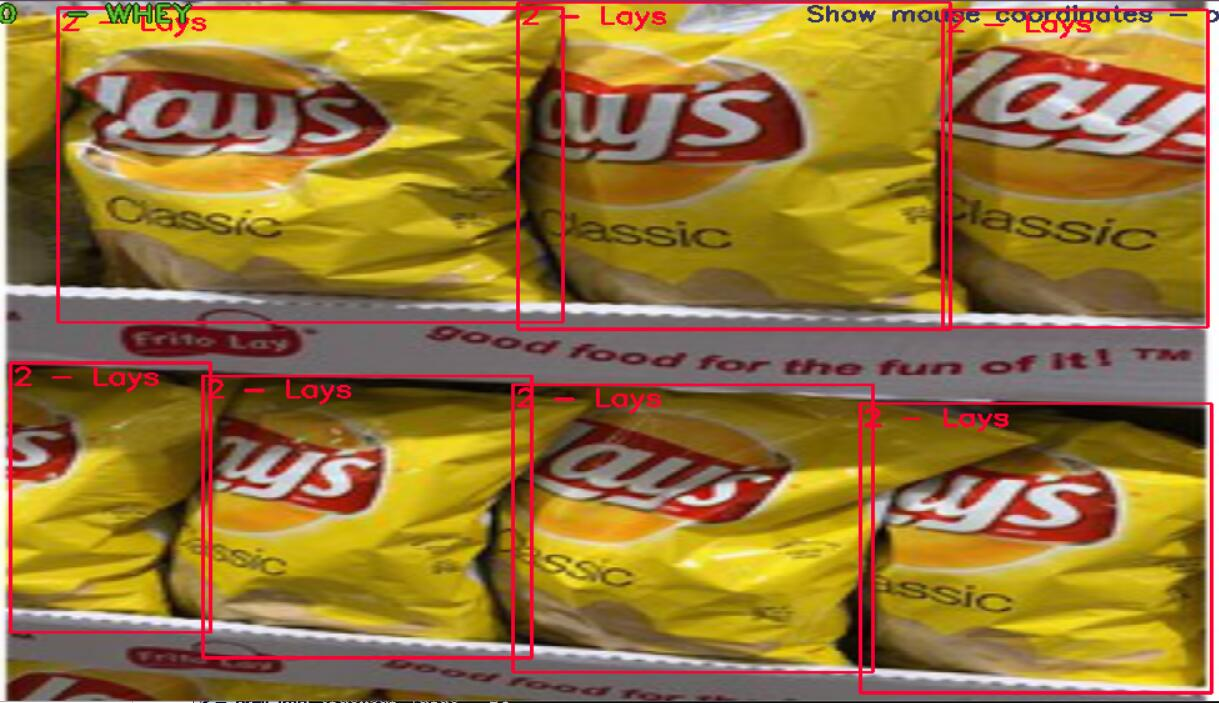
\includegraphics[width=7cm,scale=0.8]{LaysMarked.jpg}}
\caption{The test set image what we use in our experiment}
\label{fig}
\end{figure}

After marking all items, we will put all the pictures and data of the pictures into our pre-designed YOLO architecture for training.
The purpose of training is to get the weight of each item so that our system can distinguish their type and accurately judge when inputting new pictures.
In our simulator, we had 5,000 iterations of the data to get a lowest loss.
When all the data has been trained, new data can be allowed to enter.
We selected a picture that was not included in our data set to try the training results.
The category of this item is the one that has been trained by our system.
We searched the pictures of this item randomly on the Internet and put them into our system for identification.
The recognition result as shown in Fig.11

\begin{figure}[htbp]
\centerline{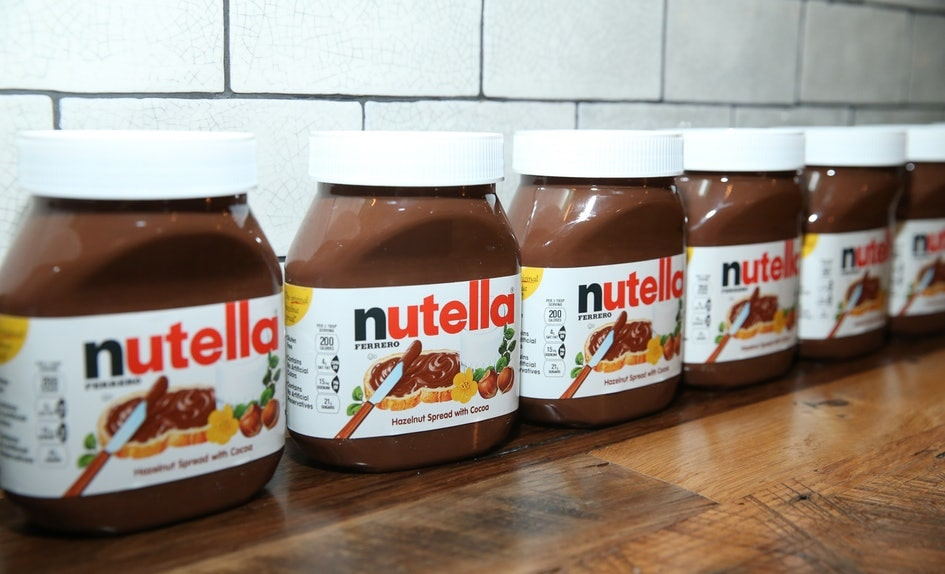
\includegraphics[width=3.5cm,scale=0.6]{nutella.jpg} 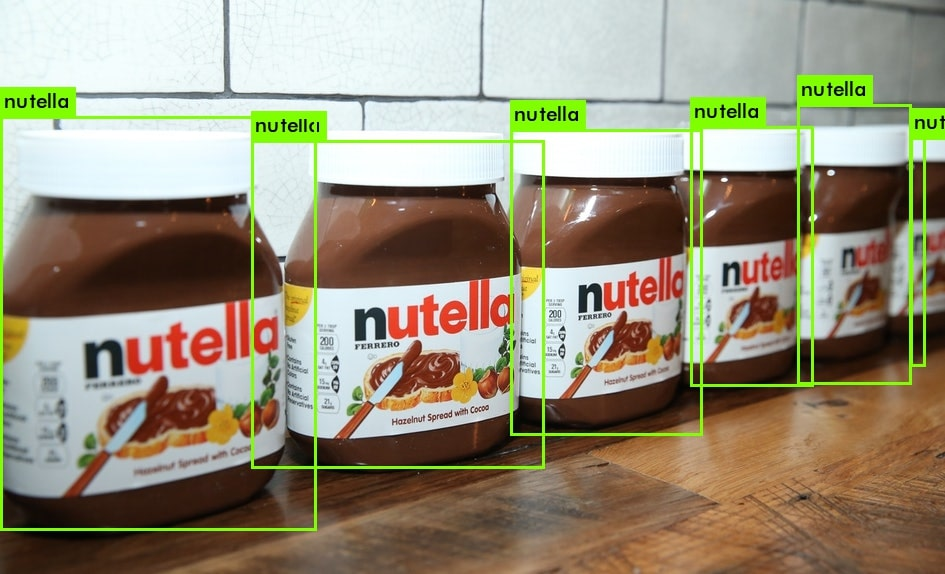
\includegraphics[width=3.5cm,scale=0.6]{nutella2.jpg}}
\caption{Put the "nutella" pictures into our recognition system and recognize the information.}
\label{fig}
\end{figure}

Our system can accurately identify the object and the number of objects in this picture, its recognition rate can reach 98\%.
This means that when the camera in the scene intercepts the picture and puts it into our system, it can accurately identify the type and number of them.
It shows that the system we built is feasible to be used in real scenes.
Ultimately we'll have it with multi cameras to achieve cashier-free supermarket.






%\begin{table}[htbp]
%\caption{Table Type Styles}
%\begin{center}
%\begin{tabular}{|c|c|c|c|}
%\hline
%\textbf{Table}&\multicolumn{3}{|c|}{\textbf{Table Column Head}} \\
%\cline{2-4}
%\textbf{Head} & \textbf{\textit{Table column subhead}}& \textbf{\textit{Subhead}}& \textbf{\textit{Subhead}} \\
%\hline
%copy& More table copy$^{\mathrm{a}}$& &  \\
%\hline
%\multicolumn{4}{l}{$^{\mathrm{a}}$Sample of a Table footnote.}
%\end{tabular}
%\label{tab1}
%\end{center}
%\end{table}



\bibliographystyle{IEEEtran}
\bibliography{refer_output}


\vspace{12pt}


\end{document}
